\section{Load Cell}
The load cell used in this project is a MP40/10 N. \cite{DS-MP40} 
It has a max. capacity of \SI{1}{\kilogram} making it suitable for a counting scale used to count small pieces, e.g. screws. 
The load cell has a rated output of \SI{1}{\milli\volt/\volt}.
The maximum supply voltage for the load cell is \SI{15}{\volt}, but it was chosen to use a \SI{5}{\volt} supply from the Arduino ATMega2560 board. 
This was done as a project delimitation to avoid using more than one voltage supply for the system. \\

The voltage output from the load cell depends on the supply voltage. 
This will require a constant voltage supply. 
To compensate for voltage dips, short interruptions or ripple in the supply voltage, a reference voltage is given to the analog reference pin, \mintinline{c}{AREF} for the ADC. 
The output is hereby ratiometric to the supply voltage.

\begin{figure}[H]
	\centering
	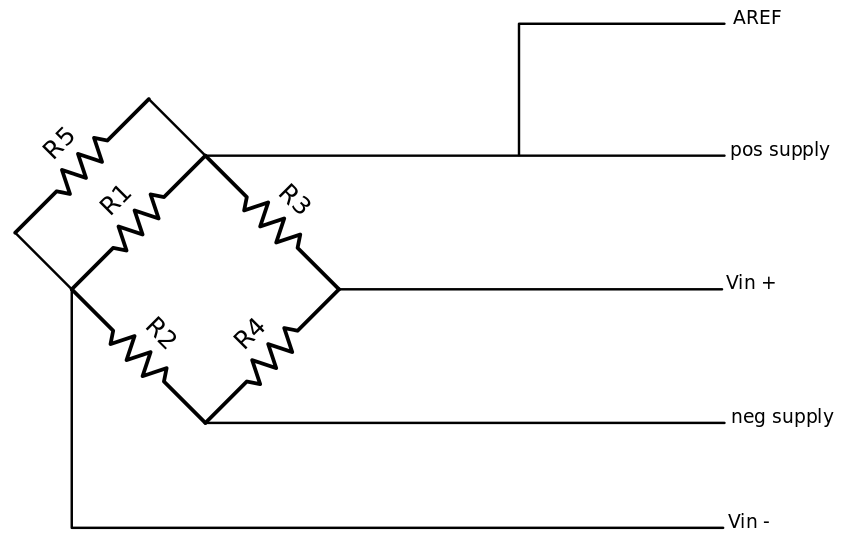
\includegraphics[width=0.6\linewidth]{graphics/loadcell}
	\caption{Ratiometric measurement.}
	\label{fig:loadcell}
\end{figure}

The load cell had an offset of $\approx\SI{28}{\milli\volt}$ at first. 
This was corrected by trimming resistor R1 in the wheatstone bridge using a parallel resistor R5 as seen on \Cref{fig:loadcell}.
When resistor R5$=\SI{51}{\kilo\hertz}$, the offset became $\approx \SI{600}{\micro\volt}$. 

\subsection{Amplifier}
With a voltage supply of \SI{5}{\volt} the output will be \SI{5}{\milli\volt}.
To use the full dynamic range of the ADC, an amplifier is needed to amplify the output.
The Arduino Atmega2560 has built-in channels for differential input with different sets of gain between $10\times$ and $200\times$.
When using $200\times$ gain, only 7 bit resolution can be expected. \cite[p.~268]{ATmega2560}
This gives a poor resolution and the gain is not sufficient to use the entire dynamic range of the ADC. 
If the gain had been selected as $200\times$, a voltage divider could have been used to lower the voltage at the \mintinline{c}{AREF} pin.
Instead of using the differential input channels with built-in gain, the instrumentation amplifier INA125P with precision voltage reference is used in this project. \cite{INA125}

\begin{equation}
G = 4+\frac{\SI{60}{\kilo\ohm}}{R_G}=\frac{\SI{60}{\kilo\ohm}}{\SI{82}{\ohm}} \approx 735
\label{eq:gain}
\end{equation}

The gain of the amplifier must be set to a value securing that the full dynamic range of the ADC is used. 
The gain of the amplifier is set to $735\times$, see \cref{eq:gain}. 
With this gain the offset becomes $\approx \SI{450}{\milli\volt}$ and will result in the ADC input range being $\approx \text{\SI{450}{\milli\volt}}+\SI{3.7}{\volt}\approx\SI{4.15}{\volt}$.
With this gain not the entire dynamic range of the ADC is used, but leaves some heading for eventually drifting. 
The gain could perhaps have been placed higher, as long the ADC input range would not exceed \SI{5}{\volt}, see \cref{eq:inputrange}.

\begin{equation}
(\text{Rated Output}+\text{Offset})\cdot G < \SI{5}{\volt}
\label{eq:inputrange}
\end{equation} 

\subsection{ADC Configuration}
The ADC converts the input voltage to a 10-bit value.
The minimum ADC value represents GND and the maximum ADC value represents the voltage on the AREF pin, minus 1 LSB.\cite[p.~269]{ATmega2560}
A single ended channel is used with the output of the instrumentation amplifier connected to \mintinline{c}{ADC0} on the Arduino ATMega2560 board. 

\paragraph{\mintinline{c}{ADMUX}} 
To select \mintinline{c}{ADC0} as input channel the \mintinline{c}{MUX} bits are set low in the \mintinline{c}{ADMUX} register.
To select \mintinline{c}{AREF} to external voltage reference, the \mintinline{c}{REFS} bits are set low.

\paragraph{\mintinline{c}{ADCSRA}}
To select the input clock to the ADC the \mintinline{c}{ADPS} bits are set high in the  \mintinline{c}{ADCSRA} register. 
These bits specify the division factor used to divide the CPU frequency. 
With a CPU frequency of \SI{16}{\mega\hertz}, a division factor of 128 will result in a input clock to the ADC of \SI{125}{\kilo\hertz}, see \cref{eq:adcclock}.
Enabling the ADC is done by writing the \mintinline{c}{ADEN} bit.

\begin{equation}
\text{ADC Clock}=\frac{\SI{16}{\mega\hertz}}{128}=\SI{125}{\kilo\hertz}
\label{eq:adcclock}
\end{equation}

\paragraph{\mintinline{c}{ADCSRB}}
To select \mintinline{c}{ADC0} as input channel the \mintinline{c}{MUX5} bit are set low in the \mintinline{c}{ADCSRB} register.\\

\noindent See datasheet for ADC register decriptions. \cite[p.~281-288]{ATmega2560}

\begin{lstlisting}[caption={Initialization of ADC.}, label={lst:ADC},language=C++,directivestyle={\color{black}},
emph={int,char,double,float,unsigned},emphstyle={\color{blue}}]
void ADC_Init()
{
	// AREF; Single Ended Input ADC0
    ADMUX = 0b00000000;
    // ADC Enable; ADC Prescaler = 128
    ADCSRA = 0b10000111;
    ADCSRB = 0b00000000;
}
\end{lstlisting}


\subsection{Count Scale Configuration}
The count scale is configured after measuring a trendline made by placing different weights upon the load cell and then reading the ADC value. 
The offset can be seen as 92 ADC counts and correspond well with the offset of \SI{450}{\milli\volt} when the ADC has a resolution of \SI{4.88}{\milli\volt}, \cref{eq:resolutionvoltage}. 
The resolution can also be specified in grams as seen in \cref{eq:resolutiongrams}.

\begin{equation}
\text{Resolution}=\frac{\SI{5}{\volt}}{2^{10}}= \SI{4.88}{\milli\volt}
\label{eq:resolutionvoltage}
\end{equation}

\begin{equation}
\text{Resolution}=\frac{\text{Weight}}{\text{ADC Count}-\text{ADC Offset}}=\frac{\SI{500}{\gram}}{462-92}=\SI{1.35}{\gram}
\label{eq:resolutiongrams}
\end{equation}

\begin{figure}[H]
	\centering
	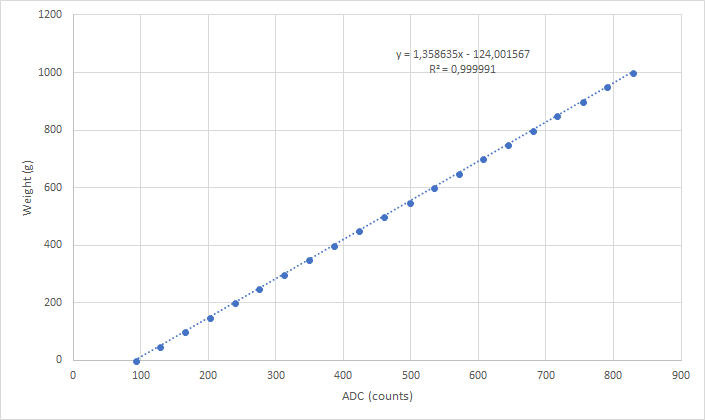
\includegraphics[width=0.67\linewidth]{graphics/loadcellconfig}
	\caption{Configuration of load cell.}
	\label{fig:loadcellconfig}
\end{figure}
\vspace{-25pt}
\begin{equation}
y = 1.3586-124
\label{eq:trendline}
\end{equation}

With this trendline, \cref{eq:trendline}, the weight corresponding to a given ADC count can be calculated.
The weight is averaged over 5 measurements to give a more steady output to avoid number flickering on the graphic display.
The amount is calculated by dividing the weight with a scaling factor given by the items weight divided by the amount of items specified by the user. 
\vspace{-15pt}
\begin{lstlisting}[caption={Amount of items calculated with use of the trendline.}, label={lst:counter},language=C++,directivestyle={\color{black}},
emph={int,char,double,float,unsigned},emphstyle={\color{blue}}]
void Counter(int ListPos)
{
	volatile int amount;
	volatile float weight;
	...
	ADC_avg += ADCW;
	count ++;
	if (count == 5)
	{
	    ADC_avg = ADC_avg / 5;
	    weight = (ADC_avg * 1.3586) - 138; // Change in offset
	    amount = (int) (weight / WeightList[ListPos]);
	    ADC_avg = 0;
	    count = 0;
	    _delay_ms(20);
	}
}
\end{lstlisting}